\section{Empirical Performance Analysis}
\label{fvgm_sec:experiments}
In this section, we empirically evaluate the performance of {\fvgm}. We first present the experimental setup and the objective of our experiments, followed by experimental results.
%\footnote{Due to page limit, we present additional experimental results, proof of lemmas, and miscellaneous details in Appendix.}

\begin{figure}[t!]
	\begin{center}		
		\subfloat{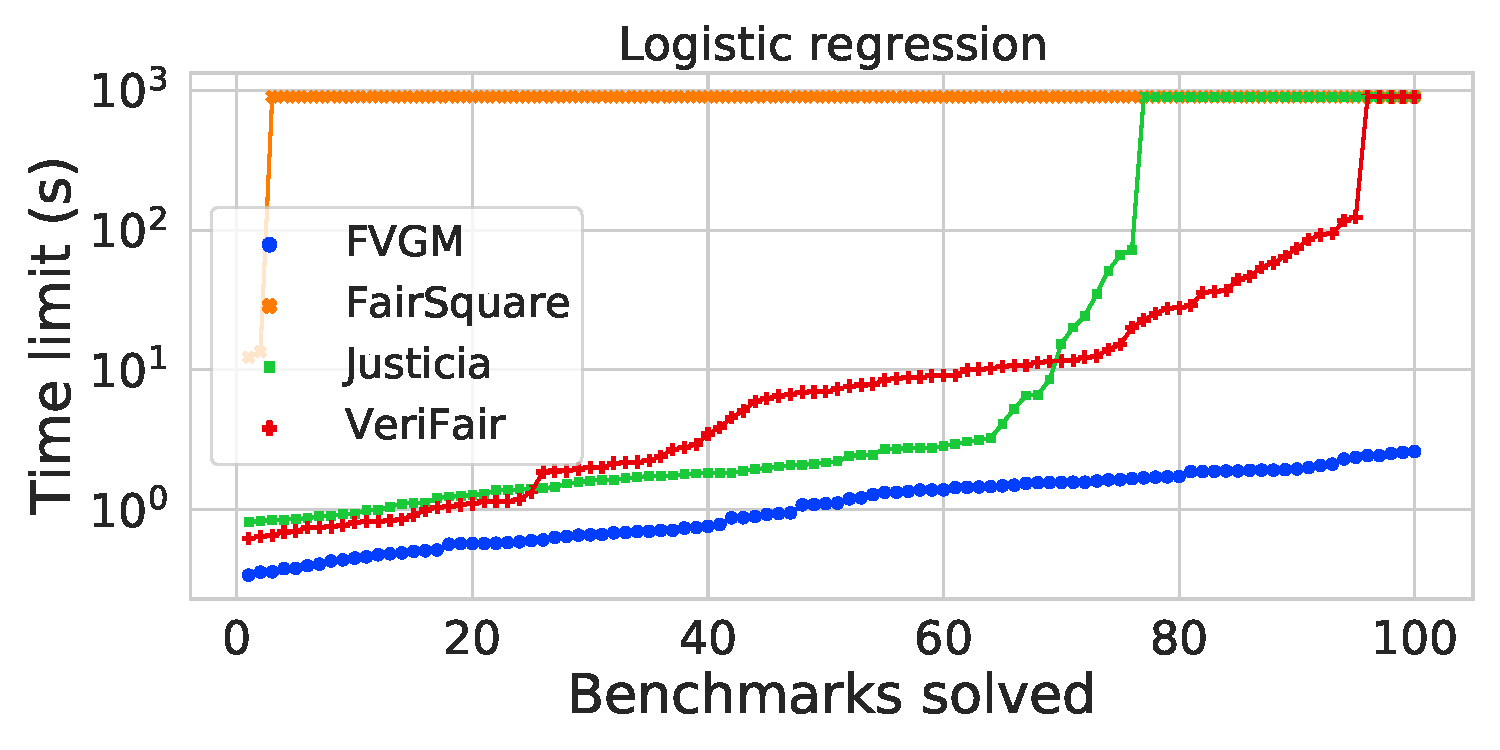
\includegraphics[scale=0.3]{figures/fairness/fvgm/cactus_all_verifiers_LR_time_}}
		\subfloat{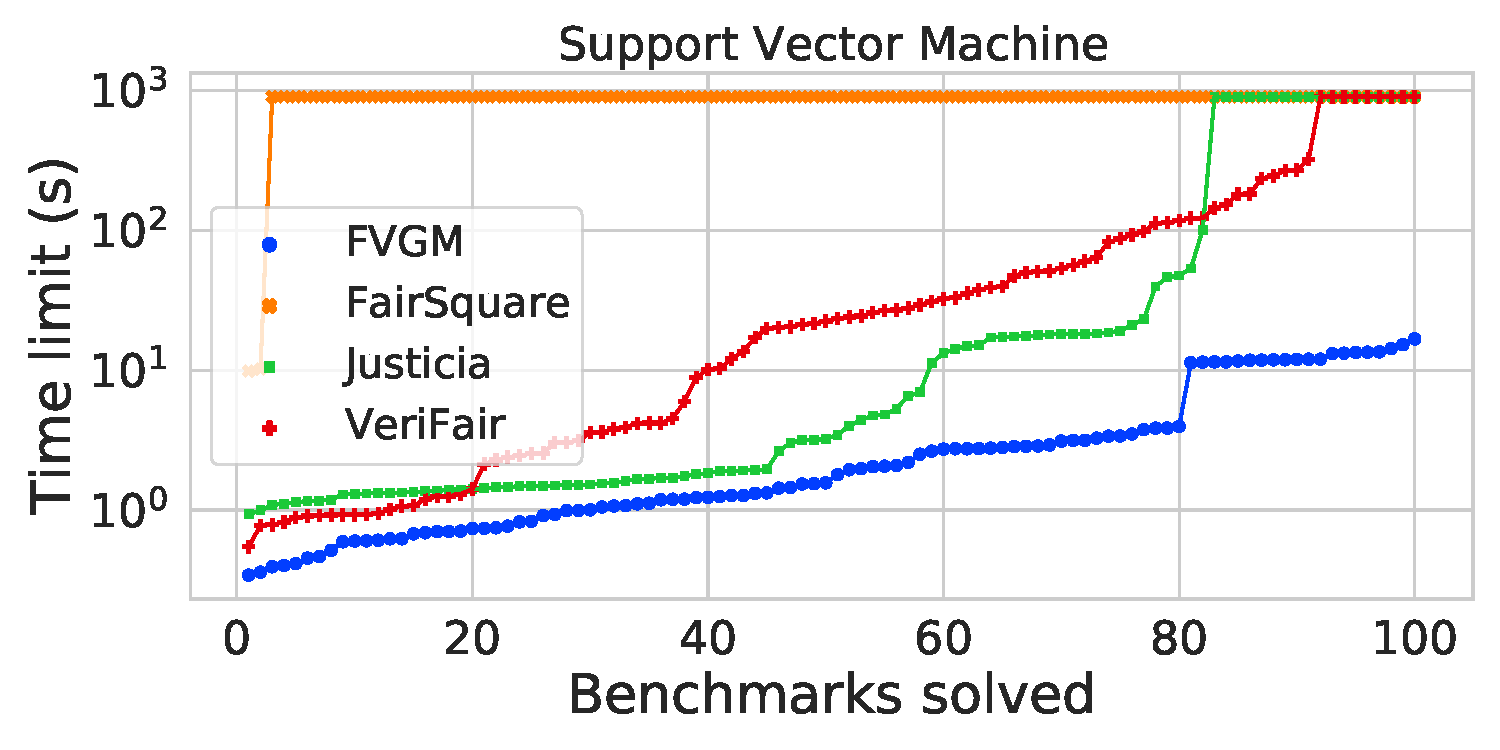
\includegraphics[scale=0.3]{figures/fairness/fvgm/cactus_all_verifiers_SVM_time_}}		
	\end{center}
	%	\vspace{-2ex}
	\caption[Scalability of {\fvgm}]{A cactus plot to present the scalability of different fairness verifiers. The number of solved benchmarks are on the $ X $-axis and the required time is on the $ Y $-axis; a point $ (x,y) $ implies that a verifier takes less than or equal to $ y $ seconds to compute fairness metrics of $ x $ many benchmarks. We consider $ 100 $ benchmarks generated from $ 5 $ real-world datasets using $ 5 $-fold cross-validation. In each fold, we consider $\{25, 50, 75, 100\} $ percent of non-sensitive features.}\label{fvgm_fig:scalability_exp}
	%	\vspace{-2ex}
\end{figure}

\textbf{Experimental Setup.}
We  implement a  prototype of {\fvgm} in Python (version 3.8).  
We deploy the Scikit-learn library for learning linear classifiers such as Logistic Regression (LR) and Support Vector Machine (SVM) with linear kernels. We perform five-fold cross-validation on a dataset. While the classifier is trained on continuous features, we discretize them to Boolean features to be invoked by {\fvgm}. During discretization, we apply a gird-search to estimate the best bin-size within a maximum bin of $ 10 $. To convert the coefficients of features into integers, we employ another grid-search to choose the best multiplier within $ \{1,2, \dots, 100\} $. For learning a Bayesian network on the converted Boolean data, we deploy the PGMPY library~\cite{ankan2015pgmpy}. For network learning, we apply a Hill-climbing search algorithm that learns a DAG structure by optimizing K2 score~\cite{koller2009probabilistic}. For estimating parameters of the network, we use Maximum Likelihood Estimation (MLE) algorithm. 

We compare {\fvgm} with three existing fairness verifiers: Justicia~\cite{ghosh2020justicia}, FairSquare~\cite{albarghouthi2017fairsquare}, and VeriFair~\cite{bastani2019probabilistic}. 
%Additionally, we have verified two fairness algorithms: reweighing algorithm (RW)~\cite{kamiran2012data} and the optimized pre-processing algorithm (OP)~\cite{calmon2017optimized}, and a fairness poisoning-attack algorithm~\cite{solans2020poisoning}. 


\subsection{Scalability Analysis}
\textbf{Benchmarks.} We perform the scalability analysis on five real-world datasets studied in fair ML literature: UCI Adult, German-credit~\cite{DK2017}, COMPAS~\cite{angwin2016machine}, Ricci~\cite{mcginley2010ricci}, and Titanic (\url{https://www.kaggle.com/c/titanic}). We consider $ 100 $ benchmarks generated from 5 real-world datasets and report the computation times (for DI and SP) of different verifiers.

\textbf{Results.} In Figure~\ref{fvgm_fig:scalability_exp}, we present the scalability results of different verifiers. First, we observe that FairSquare often times out ($ =900 $ seconds) and can solve $ \le 5 $ benchmarks. This indicates that SMT-based reduction for linear classifiers cannot scale. Similarly, SSAT-based verifier Justicia that performs pseudo-Boolean to CNF translation for linear classifiers, times out for around $  20 $ out of $ 100 $ benchmarks. Sampling-based framework, VeriFair, has comparatively better scalability than SMT/SSAT based frameworks and can solve more than $ 90 $ benchmarks. Finally, {\fvgm} achieves impressive scalability by solving all $ 100 $ benchmarks with $ 1 $ to $ 2 $ orders of magnitude runtime improvements than existing verifiers. Therefore,\textit{ {\stochastic}-based framework {\fvgm} proves to be highly scalable in verifying fairness properties of linear classifiers than the state-of-the-art.} 

\begin{figure}[t!]
	\begin{center}	
		\subfloat{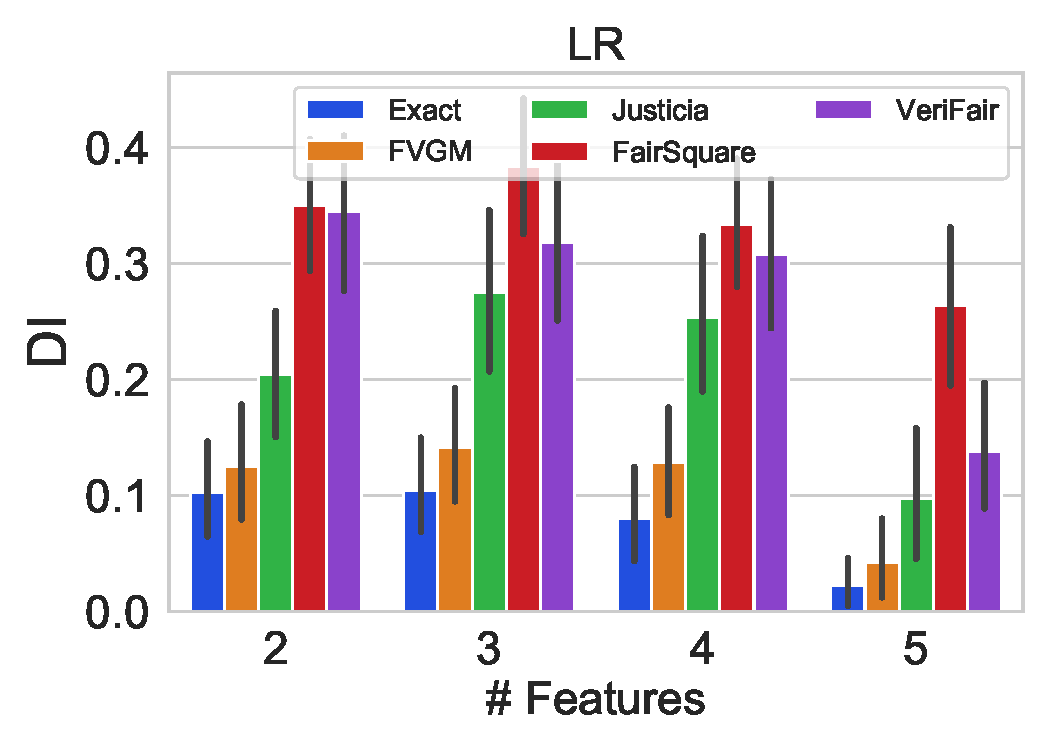
\includegraphics[scale=0.3]{figures/fairness/fvgm/sanity_DI_LR_01}}
		\subfloat{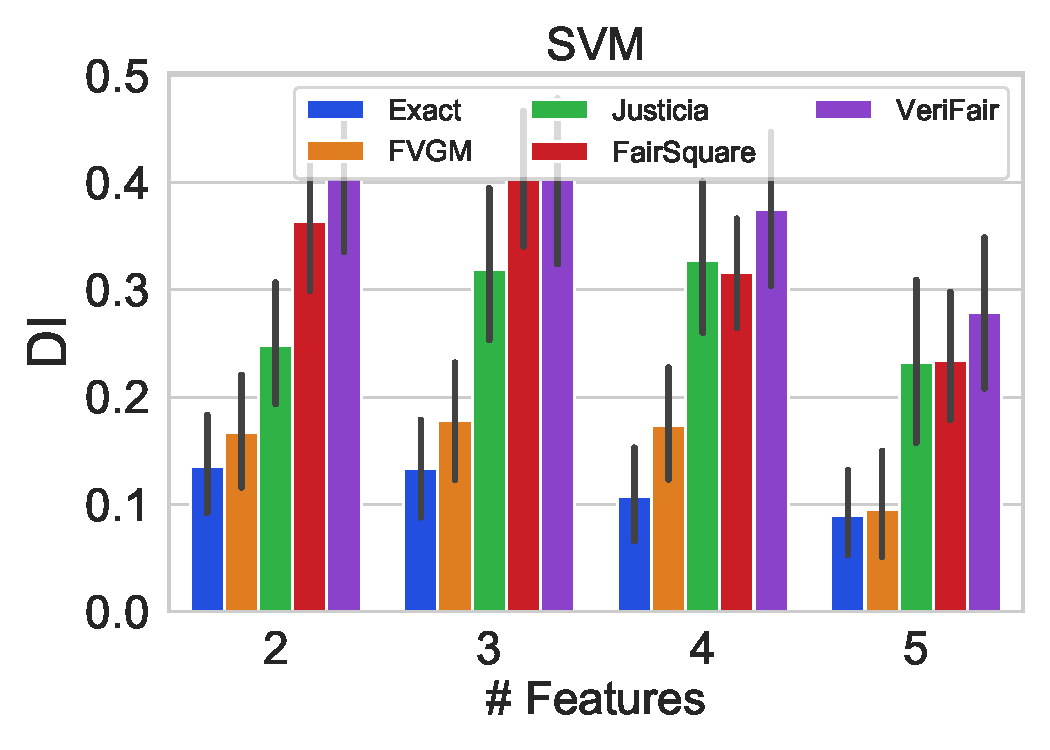
\includegraphics[scale=0.3]{figures/fairness/fvgm/sanity_DI_SVM_01}}		
		%		\subfloat[]{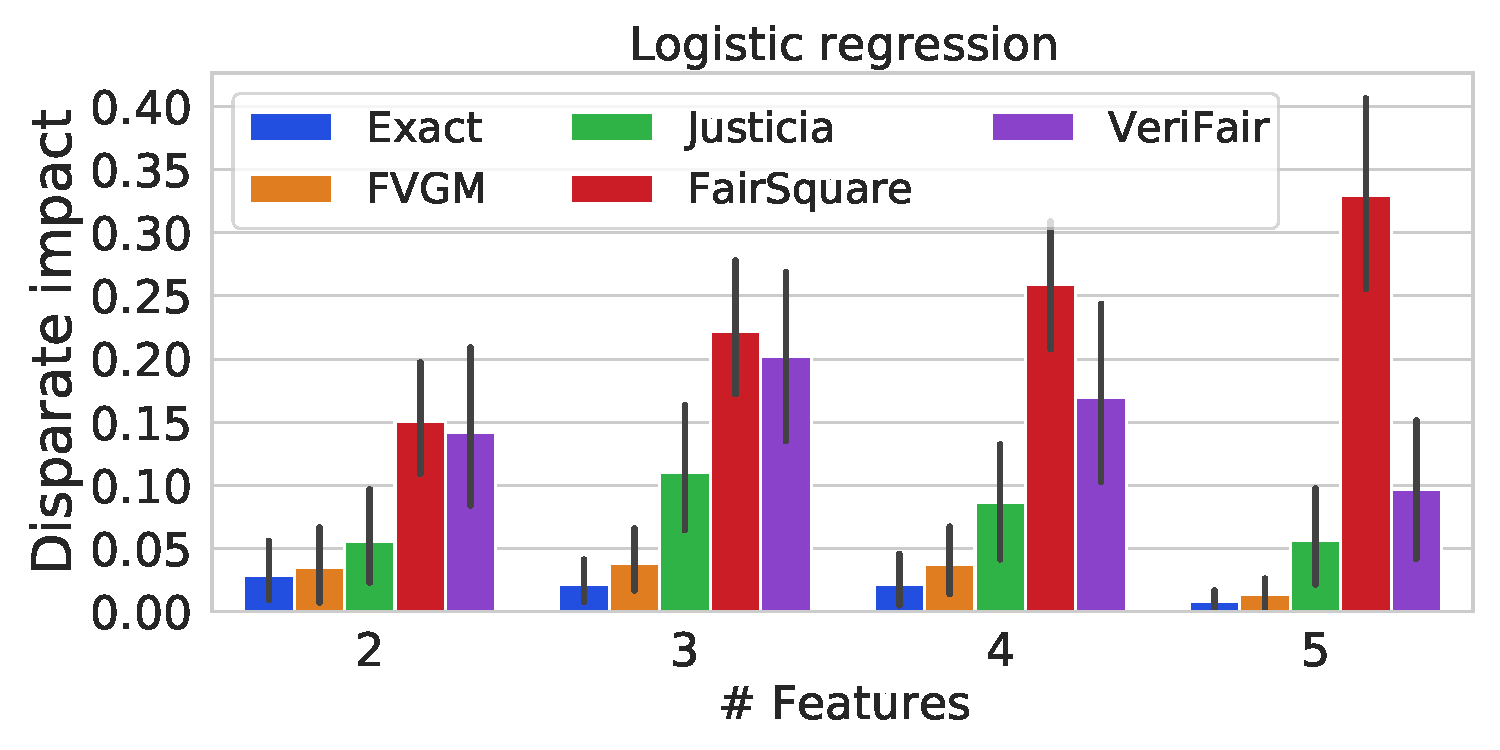
\includegraphics[scale=0.25]{figures/fairness/fvgm/sanity_DI_LR_005}}
		%		\subfloat[]{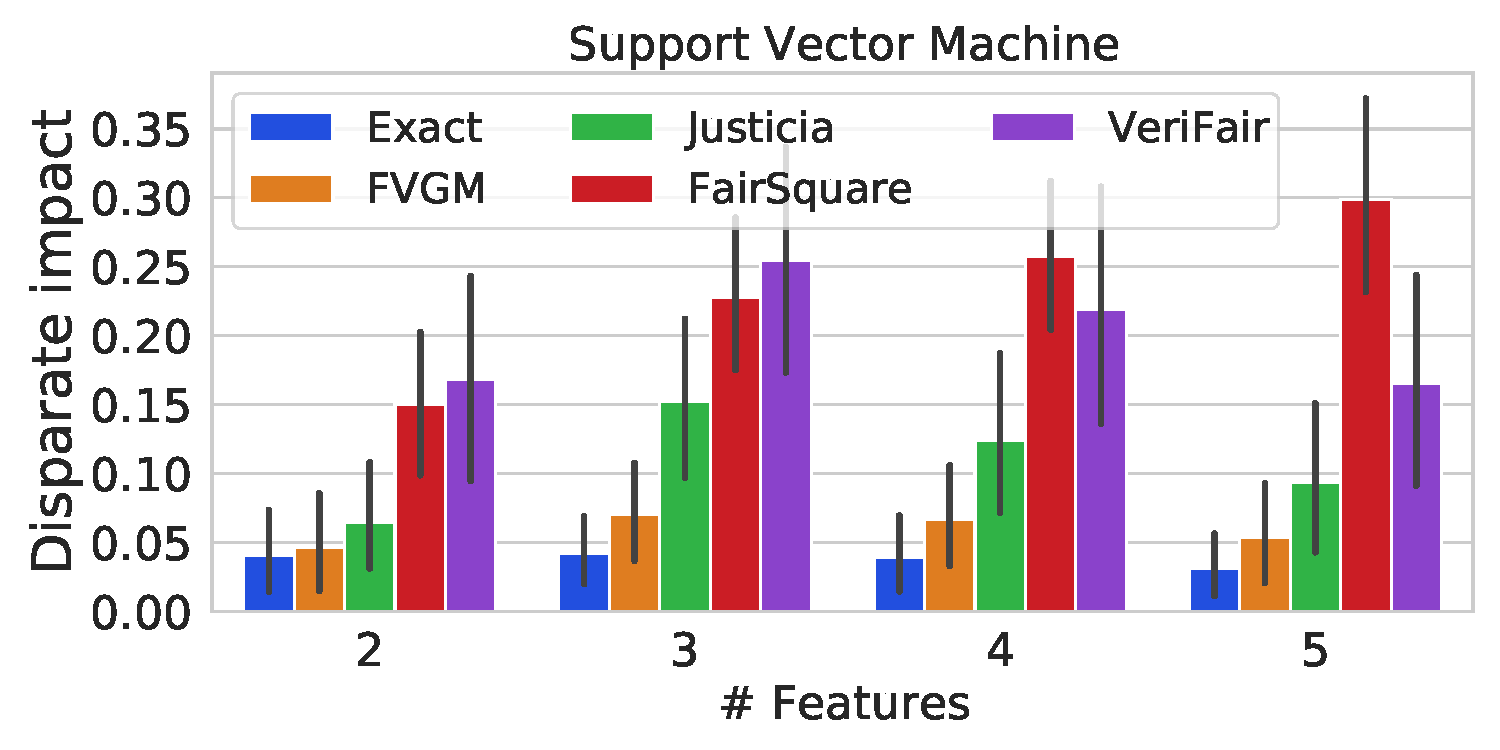
\includegraphics[scale=0.25]{figures/fairness/fvgm/sanity_DI_SVM_005}}
		%				
	\end{center}
	%	\vspace{-2ex}
	\caption[Accuracy of {\fvgm}]{Comparing the average accuracy of different verifiers over 100 synthetic benchmarks while varying the number of features. {\fvgm} yields the closest estimation of the analytically calculated \textit{Exact} values of DI for LR and SVM classifiers.}\label{fvgm_fig:sanity_exp}
	%	\vspace{-2ex}
\end{figure}
\subsection{Accuracy Analysis}
\noindent\textbf{Benchmark Generation.} To perform accuracy analysis, we require the ground truth, which is not available for real-world instances. Therefore, we focus on generating synthetic benchmarks for analytically computing the ground truth of different fairness metrics, such as DI, from the known distribution of features. In each benchmark, we consider $ n \in \{2, 3, 4, 5\} $ features including one Boolean sensitive feature, say $ A $, generated from a Bernoulli distribution with mean $ 0.5 $.  We generate non-sensitive features $ X_i $ from Gaussian distributions such that   $ \Pr[X_i | A = 1] \sim \mathcal{N}(\mu_i, \sigma^2) $ and $ \Pr[X_i | A = 0] \sim \mathcal{N}(\mu_i', \sigma^2) $, where $ \mu_i, \mu_i' \in [0,1] $, $ \sigma = 0.1 $, and $ \mu_i, \mu_i' $ are chosen from a uniform distribution in $ [0,1] $. Finally, we create label $ Y = \mathds{1}[ \sum_{i=1}^{n-1} X_i \ge 0.5 \sum_{i=1}^{n-1} (\mu_i + \mu_i')] $ such that $ Y $ does not directly depend on the sensitive feature. For each $ n $, we generate $ 100 $ random benchmarks, learn LR and SVM classifiers on them, and compute DI using different verifiers.

  
To analytically compute DI, let the coefficients of the classifier be $ w_i $ for $ X_i $ and $ w_A $ for $ A $, and bias be $ \tau $. Since all non-sensitive features are from Gaussian distributions, we compute the probability of the predicted class $ \Pr[\hat{Y} | A = 1]  \sim \mathcal{N}(\sum_{i=1}^{n-1}w_i\mu_i, \sigma_{\hat{Y}}^2) $ and $ \Pr[\hat{Y} | A = 0]  \sim \mathcal{N}(\sum_{i=1}^{n-1}w_i\mu_i', \sigma_{\hat{Y}}^2) $ with $ \sigma_{\hat{Y}}^2 =   (\sum_{i=1}^{n-1}w_i^2)\sigma^2 $. Hence, the probability of positive prediction of the classifier  is $  1 - \mathsf{CDF}_{\hat{Y}| A =1}(\tau - w_A) $ for $ A = 1 $ and $  1 - \mathsf{CDF}_{\hat{Y}|A=0}(\tau) $ for $ A = 0 $, where $ \mathsf{CDF} $ is the cumulative distribution function. Finally, we compute DI by taking the ratio of the minimum and the maximum of the probability of positive prediction of the classifier.



\textbf{Results.} 
%\begin{enumerate}[leftmargin=*]
%	\itemsep0em 
%	\item How \textit{accurate} is {\fvgm} w.r.t. existing verifiers?
%	\item How \textit{scalable} is {\fvgm} w.r.t. existing verifiers?
%	%\item Can {\fvgm} be applied to fairness problems such as \textit{verifying} different \textit{fairness metric}s for different \textit{fair ML algorithms} and \textit{fairness attacks}, and also \textit{detecting the sources of bias} due to different subset of features?
%\end{enumerate}
%To summarize our experimental results, {\fvgm} is more accurate and scalable than existing fairness verifiers in verifying linear classifiers on benchmark datasets. %{\fvgm} can verify diverse set of fairness metrics for multiple fairness-enhancing algorithms and depreciation attacks. {\fvgm} also computes fairness influence functions that can detect bias in the level of individual features. 
%\red{Due to limited space, we discuss additional experiments including verification of CNF-based classifiers with feature correlations and performance analysis of encoding Bayesian networks in Appendix.}
 We  assess the accuracy of the competing verifiers in estimating fairness metrics, specifically DI with LR and SVM classifiers. In Figure~\ref{fvgm_fig:sanity_exp}, {\fvgm} computes DI closest to the \textit{Exact} value for different number of features and both type of classifiers. In contrast, Justicia, FairSquare, and VeriFair measure DI far from the \textit{Exact} because of ignoring correlations among the features. For example, for SVM classifier with  $ n = 5 $ (right plot in Figure~\ref{fvgm_fig:sanity_exp}), \textit{Exact} DI is $ 0.089 $ (average over 100 random benchmarks). Here, {\fvgm} computes DI as $ 0.094 $, while all other verifiers compute DI as at least $ 0.233 $. Therefore, \textit{{\fvgm} is more accurate than existing verifiers as it explicitly considers correlations among features}. 








\begin{table}[!t]
	
	\caption[Verification of fairness metrics and algorithms using {\fvgm}]{Verification of fairness algorithms using {\fvgm}. $ \sensitive $ denotes sensitive features.  RW and OP refer to reweighing and optimized-preprocessing algorithms. Numbers in bold refer to fairness improvement.   }\label{fvgm_tab:fair_algo_verification}
	
		\centering
		
		
%		\setlength{\tabcolsep}{0.45em}
		\begin{tabular}{lllrrrrrrrrrrrrr}
			
			\toprule
			Dataset & $ \sensitive $ & Algo. & $ \Delta $DI &  $ \Delta $PCF & $ \Delta $SP & $ \Delta $EO\\
			\midrule
			
			
			\multirow{4}{*}{\rotatebox[origin=c]{0}{Adult}}&\multirow{2}{*}{\rotatebox[origin=c]{0}{race}}&RW&$ \textbf{0.53} $&$ \textbf{-0.06} $&$ \textbf{-0.06} $&$ \textbf{-0.02} $\\
			&&OP&$ \textbf{0.57} $&$ \textbf{-0.07} $&$ \textbf{-0.07} $&$ \textbf{-0.02} $\\
			\cmidrule{2-7}
			&\multirow{2}{*}{\rotatebox[origin=c]{0}{sex}}&RW&$ \textbf{0.96} $&$ \textbf{-0.16} $&$ \textbf{-0.15} $&$ \textbf{-0.08} $\\
			&&OP&$ \textbf{0.43} $&$ \textbf{-0.08} $&$ \textbf{-0.08} $&$ 0.03 $\\
			
			
			\midrule
			\multirow{4}{*}{COMPAS}&\multirow{2}{*}{race}&RW&$ \textbf{0.13} $&$ \textbf{-0.07} $&$ \textbf{-0.07} $&$ \textbf{-0.06} $\\
			&&OP&$ \textbf{0.15} $&$ \textbf{-0.08} $&$ \textbf{-0.08} $&$ \textbf{-0.05} $\\
			\cmidrule{2-7}
			&\multirow{2}{*}{sex}&RW&$ \textbf{0.1} $&$ \textbf{-0.04} $&$ \textbf{-0.04} $&$ 0.04 $\\
			&&OP&$ \textbf{0.09} $&$ \textbf{-0.04} $&$ \textbf{-0.04} $&$ \textbf{-0.03} $\\
			
			\midrule
			\multirow{4}{*}{German}&\multirow{2}{*}{age}&RW&$ \textbf{0.52} $&$ \textbf{-0.53} $&$ \textbf{-0.52} $&$ \textbf{-0.47} $\\
			&&OP&$ \textbf{0.53} $&$ \textbf{-0.53} $&$ \textbf{-0.53} $&$ \textbf{-0.51} $\\
			\cmidrule{2-7}
			&\multirow{2}{*}{sex}&RW&$ -0.06 $&$ 0.06 $&$ 0.06 $&$ 0.02 $\\
			&&OP&$ -0.12 $&$ 0.12 $&$ 0.12 $&$ 0.07 $\\
			
			
			\bottomrule
		\end{tabular}
	
	
		
		
	
\end{table}









%\begin{table}[!t]
%	\begin{minipage}{0.6\columnwidth}
%		\centering
%		\small
%		
%		\setlength{\tabcolsep}{.25em}
%		
%		\begin{tabular}{lllrrrrrrrrrrrrr}
%			
%			\toprule
%			$\mathbf{D}$ & $ \sensitive $ & Algo. & $ \Delta $DI &  $ \Delta $PCF & $ \Delta $SP & $ \Delta $EO\\
%			\midrule
%			
%			
%			\multirow{4}{*}{\rotatebox[origin=c]{90}{Adult}}&\multirow{2}{*}{\rotatebox[origin=c]{90}{race}}&RW&$ \textbf{0.53} $&$ \textbf{-0.06} $&$ \textbf{-0.06} $&$ \textbf{-0.02} $\\
%			&&OP&$ \textbf{0.57} $&$ \textbf{-0.07} $&$ \textbf{-0.07} $&$ \textbf{-0.02} $\\
%			\cmidrule{2-7}
%			&\multirow{2}{*}{\rotatebox[origin=c]{90}{sex}}&RW&$ \textbf{0.96} $&$ \textbf{-0.16} $&$ \textbf{-0.15} $&$ \textbf{-0.08} $\\
%			&&OP&$ \textbf{0.43} $&$ \textbf{-0.08} $&$ \textbf{-0.08} $&$ 0.03 $\\
%			
%			\bottomrule
%		\end{tabular}
%		
%		\caption{\footnotesize Verification of fairness algorithms using {\fvgm}. $ \mathbf{D} $ and $ \sensitive $ denote dataset and sensitive features.  RW and OP refer to reweighing and optimized-preprocessing algorithms. Numbers in bold refer to fairness improvement.   }\label{fvgm_tab:fair_algo_verification}
%		
%	\end{minipage}\hspace*{1em}
%	\begin{minipage}{0.4\columnwidth}
%		\centering
%		\subfloat{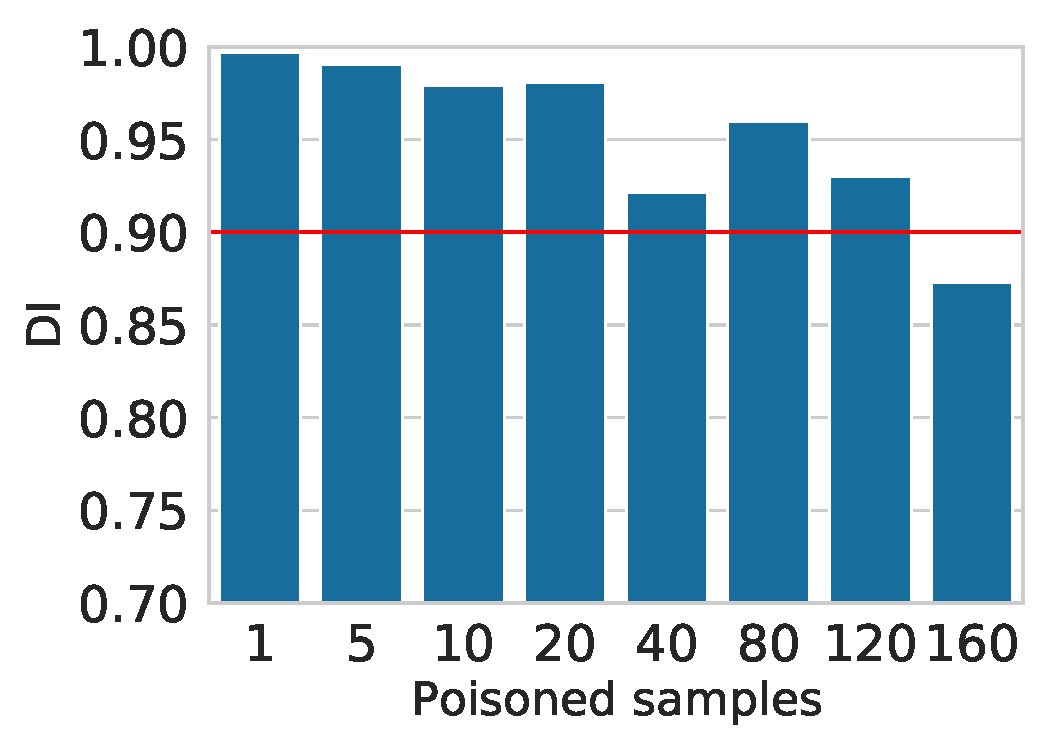
\includegraphics[scale=0.2]{figures/fairness/fvgm/disp_fairness_attack}}
%		\captionof{figure}{\footnotesize Verifying poisoning attack against fairness using {\fvgm}. The red line denotes the safety margin of the ML model against the attack.}\label{fvgm_fig:fairness_attacks}
%	\end{minipage}\hspace*{1em}
%%	\vspace{-2ex}
%	
%\end{table}

